\chapter{Grundlagen} \label{Grundlagen}

%Kurze Erläuterung der Aufgabenstellung und der Messmethode, d.h. stichwortartige 
%Zusammenstellung von wesentlichen Definitionen, Formeln, etc. (keine Herleitungen, 
%keine seitenlange Darstellung von Lehrbuchwissen!). 


\begin{figure}[h]
    \centering
    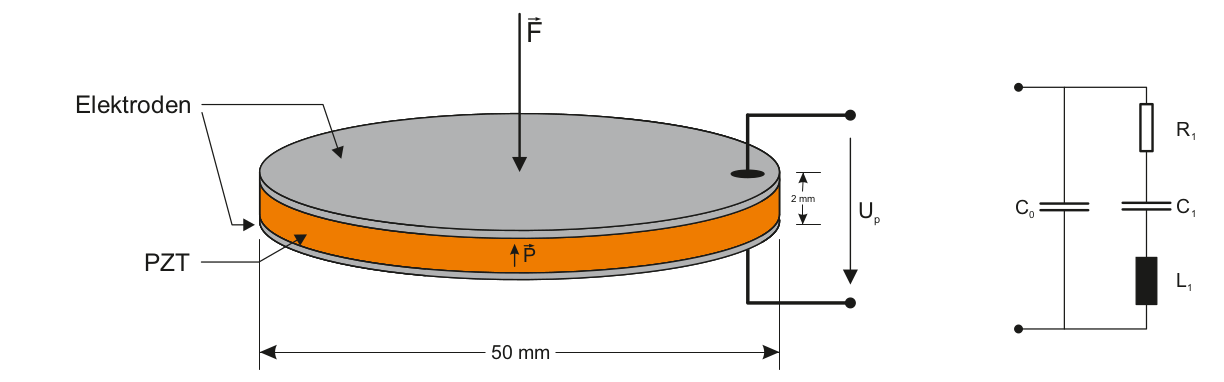
\includegraphics[width=1 \textwidth]{image/Piezo_Skizze.png}
    \caption{Piezoelektrische Scheibe mit Ersatzschaltbild  \cite{laborpraktikum2022} }
    \label{img:Ersartzschaltbild}
\end{figure}




